\chapter{CellTAN Application} \label{chap:chap5}


\section{Case study}


The experiments validating CellTAN's behavior incorporate two neighboring grid-tied string inverters from the same PV farm with common satellite data. Their only known characteristics are:

\begin{itemize}
    \item Inverter one: 12.5kW nominal power, 14.4kW peak power. Installed January 1st, 2013.
    \item Inverter two: 15kW nominal power, 15.84kW peak power. Installed January 1st, 2013.
\end{itemize}

\begin{table}[h!]
\caption{Available variables from two inverters and a satellite.}
\label{tab:availablevariables}
\resizebox{\textwidth}{!}{%
\begin{tabular}{|l|l|l|l|}
\hline
\multicolumn{1}{|c|}{\textbf{Variable}} & \multicolumn{1}{c|}{\textbf{Source}} & \multicolumn{1}{c|}{\textbf{Unit}} & \multicolumn{1}{c|}{\textbf{Label}} \\ \hline
AC side power                           & Inverter (1 \& 2)                    & W                                  & ac\_power                           \\ \hline
AC side current                         & Inverter (1 \& 2)                    & A                                  & ac\_current                         \\ \hline
AC side voltage                         & Inverter (1 \& 2)                    & V                                  & ac\_voltage                         \\ \hline
DC side power                           & Inverter (1 \& 2)                    & W                                  & dc\_power                           \\ \hline
DC side current                         & Inverter (1 \& 2)                    & A                                  & dc\_current                         \\ \hline
DC side voltage                         & Inverter (1 \& 2)                    & V                                  & dc\_voltage                         \\ \hline
Global tilted irradiance                & Satellite                            & W/m\textasciicircum{}2             & global\_tilted\_irradiance          \\ \hline
Global horizontal irradiance            & Satellite                            & W/m\textasciicircum{}2             & global\_horizontal\_irradiance      \\ \hline
Cloud coverage                          & Satellite                            & \%                                 & cloud\_coverage                     \\ \hline
Air temperature                         & Satellite                            & ºC                                 & temperature                         \\ \hline
\end{tabular}%
}
\end{table}

Table \ref{tab:availablevariables} represents the available variables and corresponding labels used to identify them in the cell's inputs and graphs. These variables are sampled every 10 minutes from May 31, 2020, at 5:00 am to April 30, 2023, at 7:30 pm (although having some gaps). We utilized data from 2020 until the end of 2022 for the cells' knowledge base, and any information from 2023 onwards is considered new and used for testing. Since there is no production at night, the database does not store values for this period. Not accounting for the night as missing samples, we have around 98\% of data availability.

Analyzing and cleaning raw inverter and satellite data is essential to take full benefit of CellTAN's capabilities. As seen in its development, having a clean knowledge base contributes to correctly identifying anomalous situations. Therefore, the following sections focus on these two steps, contributing to understanding the anomalies' domain and frequency of occurrence.

\subsection{Data analysis}

Before data visualization, and regarding the variables in table \ref{tab:availablevariables}, we eliminate those that will not benefit the CellTAN. We determined that AC side voltage is insignificant since the grid mandates it in a grid-tied inverter. We have decided to only use the measure of power instead of using the AC side current measure since, in conjunction with voltage, it provides the same information. To simplify things further, we do not need to consider the power on the DC if considering both the DC side current and voltage measures.

We examine all variables related to satellite data to determine which ones could be useful, not making any premature assumptions.

\subsubsection{Power}


\begin{figure}[h!]
    \centering
    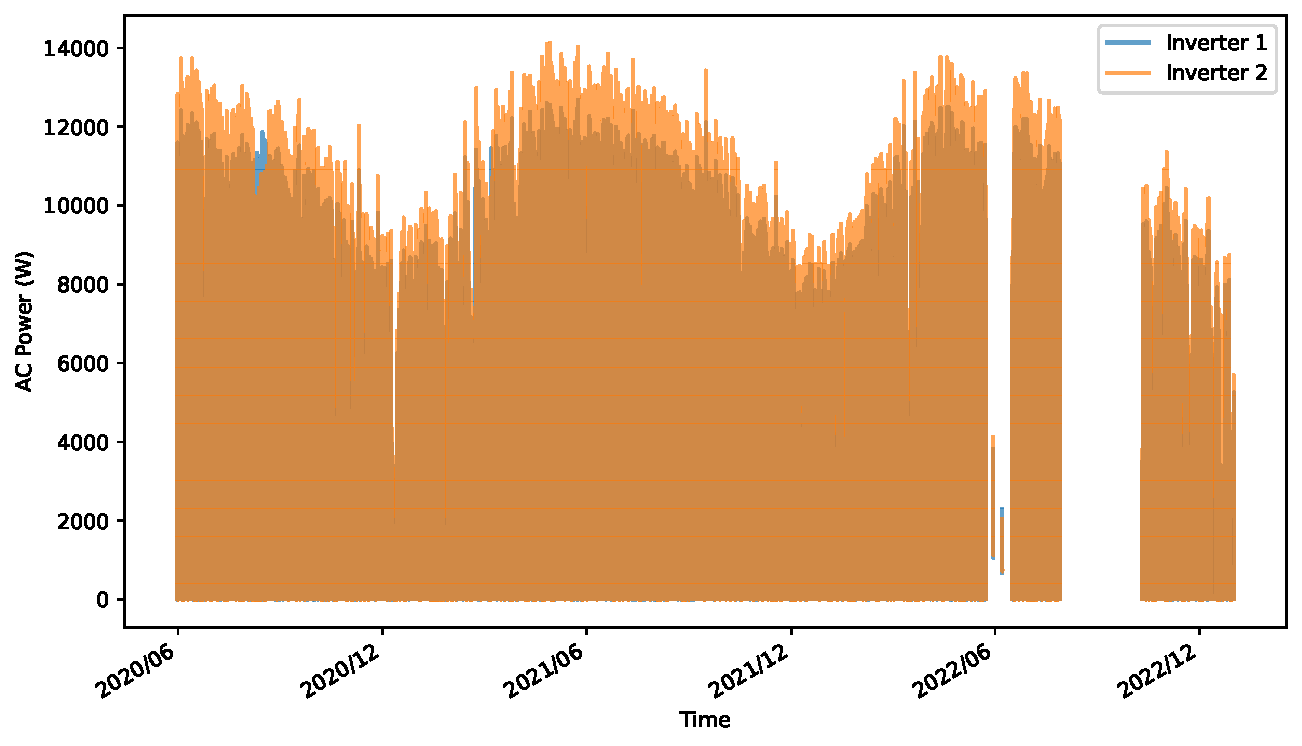
\includegraphics[width=\textwidth]{figures/chapter5/analysis/00_power_kb.pdf}
    \caption{Inverter AC side power from 2020 to 2022, used for the knowledge base.}
    \label{fig:eda_power_kb}
\end{figure}

Figure \ref{fig:eda_power_kb} shows the power profile of the two studied inverters. Right away, we notice that the power of inverter two caps at around 14kW, while inverter one usually maxes at 12kW. This information is coherent with their ratings. We can notice two relatively large chunks of missing data, with the gaps occurring in mid to late 2022.

\begin{figure}[h!]
    \centering
    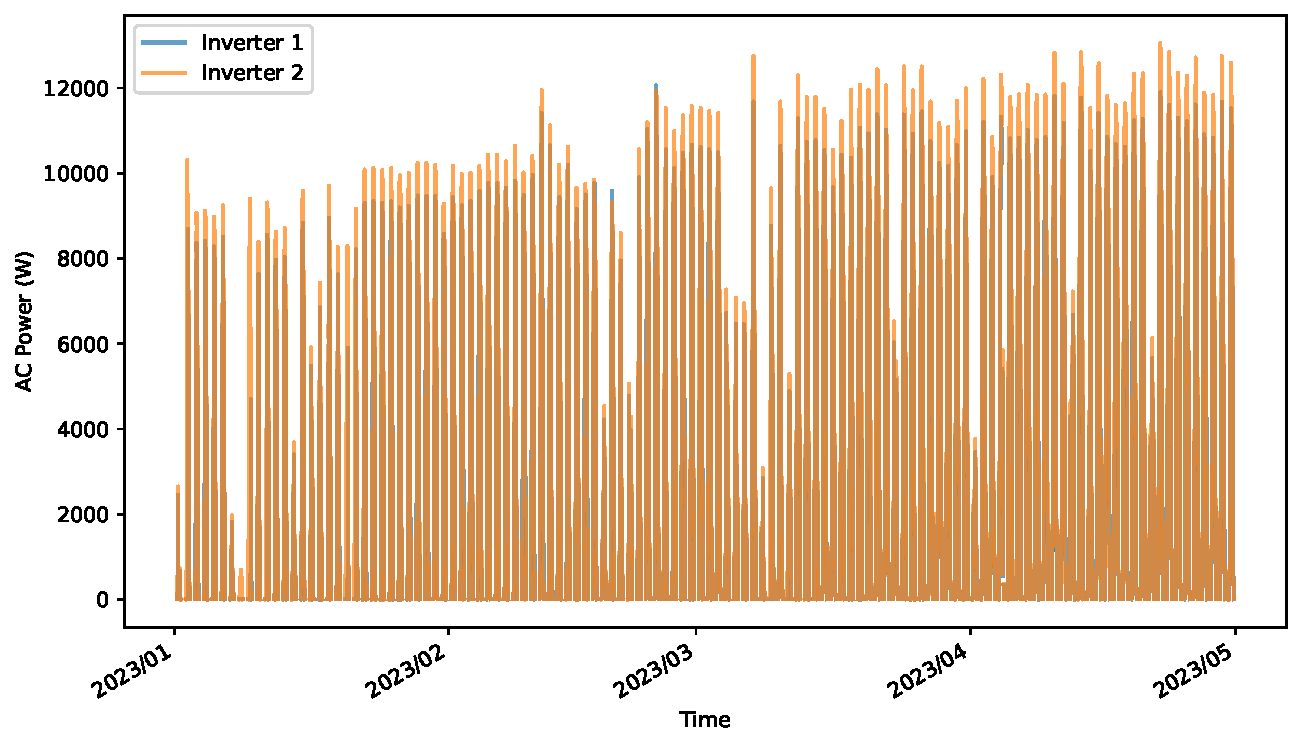
\includegraphics[width=\textwidth]{figures/chapter5/analysis/01_power_test.pdf}
    \caption{Inverter AC side power from 2023-01-01 to 2023-01-05, used for testing.}
    \label{fig:eda_power_test}
\end{figure}

Figure \ref{fig:eda_power_test} represents the power profile on the portion of data used for testing. When performing a closer inspection (with more zoom), we could hand-pick some fault occurrences in both datasets, with the majority being one inverter off while the other continues regular operation. However, these will be more noticeable during different types of data analysis, such as pair plotting. Regardless, the cases that will matter are in the test data since these scenarios will not exist in the knowledge after cleaning. In Section \ref{subsec:results}, you will find a selection of carefully chosen scenarios.

\begin{figure}[h!]
    \centering
    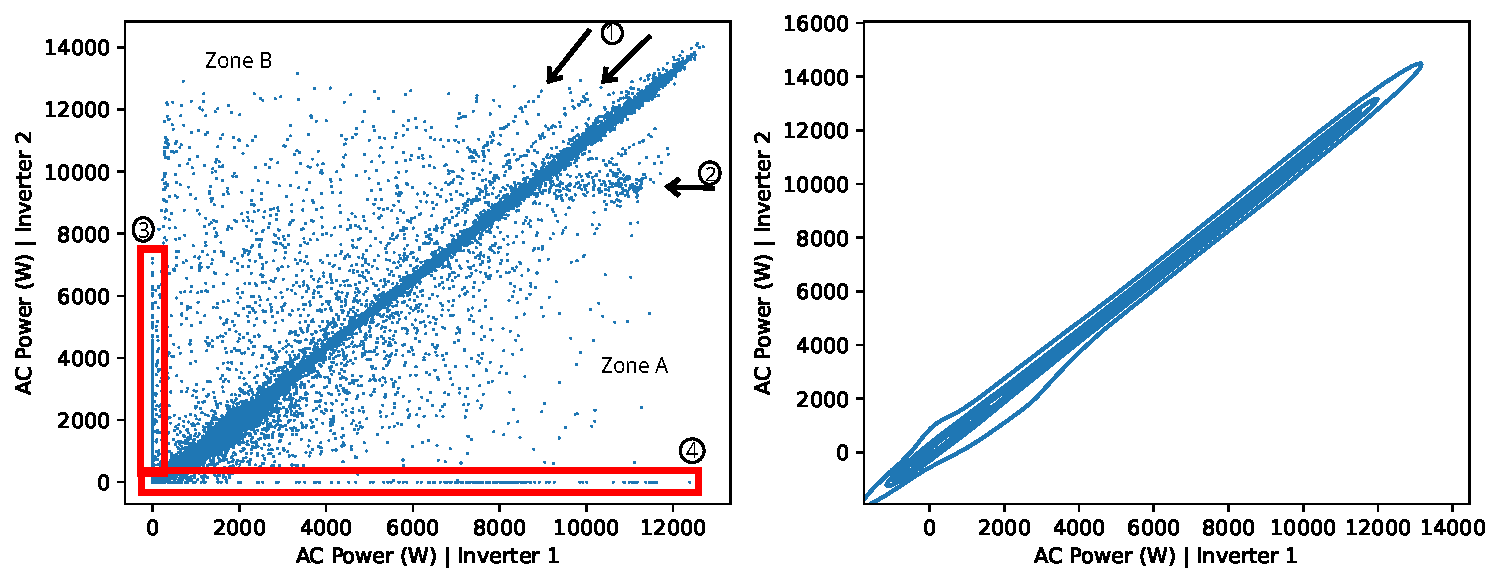
\includegraphics[width=\textwidth]{figures/chapter5/analysis/02_power_pairplots_kb.pdf}
    \caption{Pair plot of AC power from both inverters (2020 to 2022), using scatter (left) and KDE (Kernel Density Estimation) (right).}
    \label{fig:eda_power_kb_pair}
\end{figure}

% escrever sobre fig. Falar do que as zonas acima e abaixo da linha de tendencia central representam zonas de sub desempenho de um dos inversores, e mencionar as linhas de tendencia secundárias. Este pdf devia levar umas setas vermelhas ou algo do género a apontar às outras linhas de tendência.
% meter em anexos o pairplot de teste

\begin{figure}[h!]
    \centering
    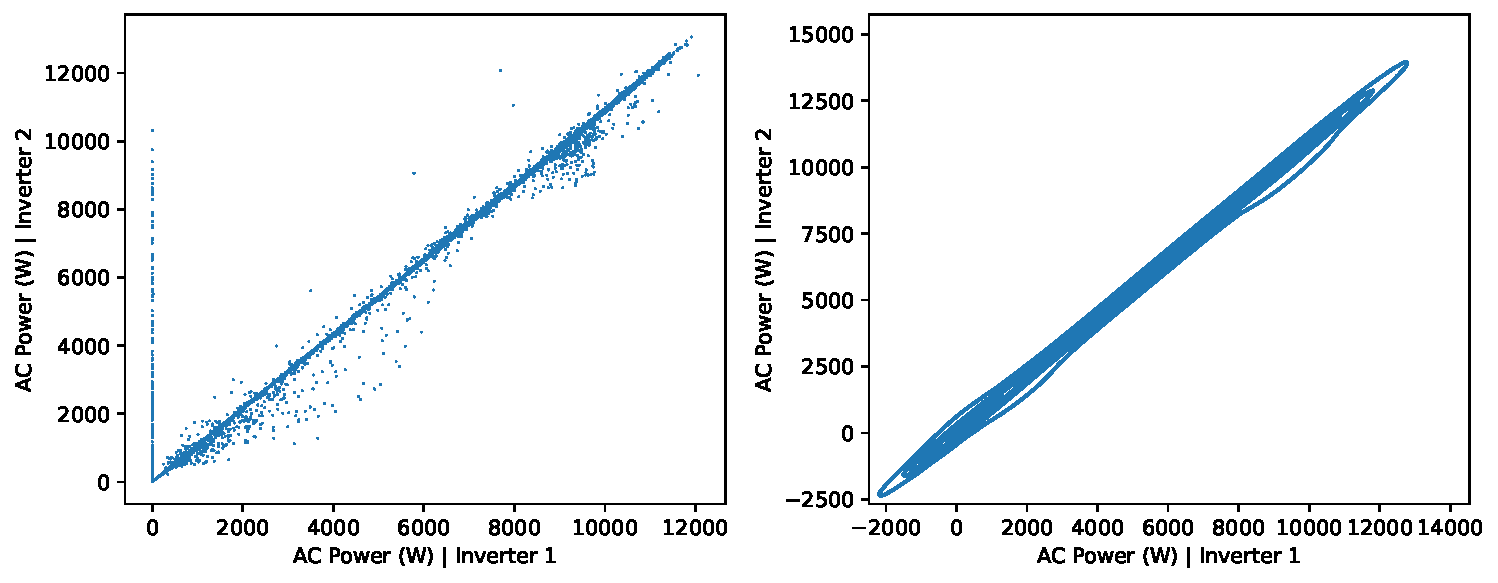
\includegraphics[width=\textwidth]{figures/chapter5/analysis/03_power_pairplots_test.pdf}
    \caption{Pair plot of AC power from both inverters (2023), using scatter (left) and KDE (Kernel Density Estimation) (right).}
    \label{fig:eda_power_test_pair}
\end{figure}

% dizer que tem menos outliers, mas várias situações com o inversor 1 inoperacional

\subsubsection{Voltage and Current}

\begin{figure}[h!]
    \centering
    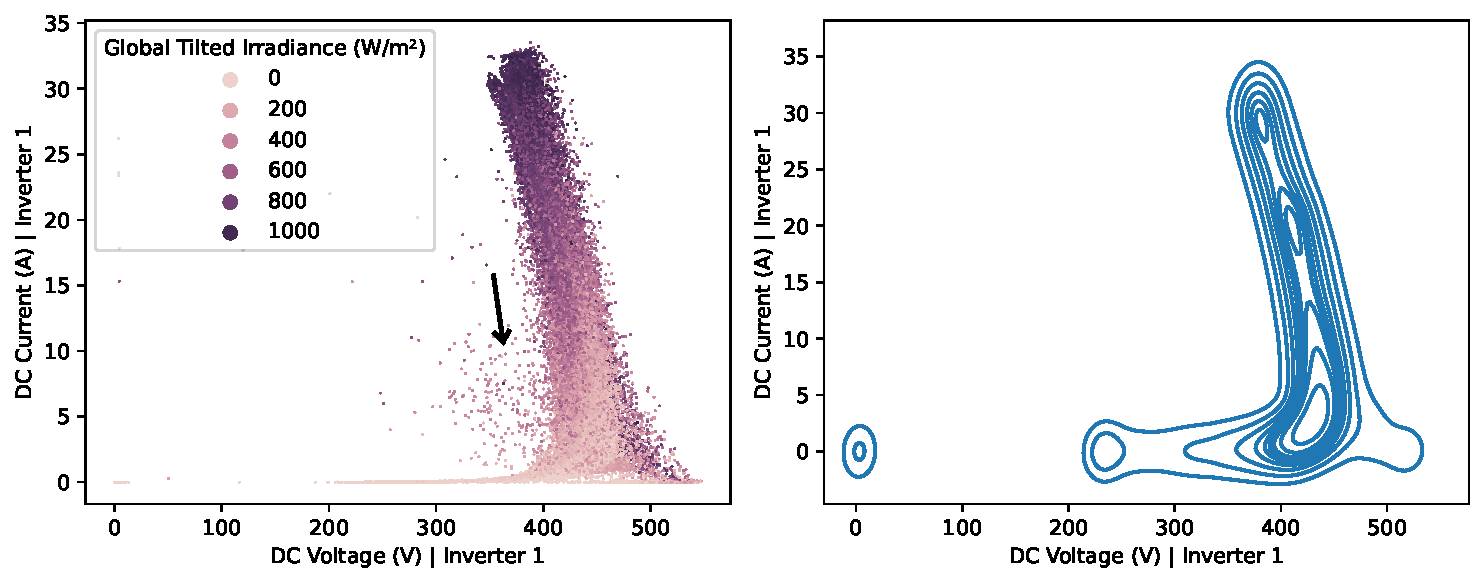
\includegraphics[width=\textwidth]{figures/chapter5/analysis/04_voltage_current_pairplot_kb_1.pdf}
    \caption{\dots}
    \label{fig:eda_volt_curr_pair_kb_1}
\end{figure}

\begin{figure}[h!]
    \centering
    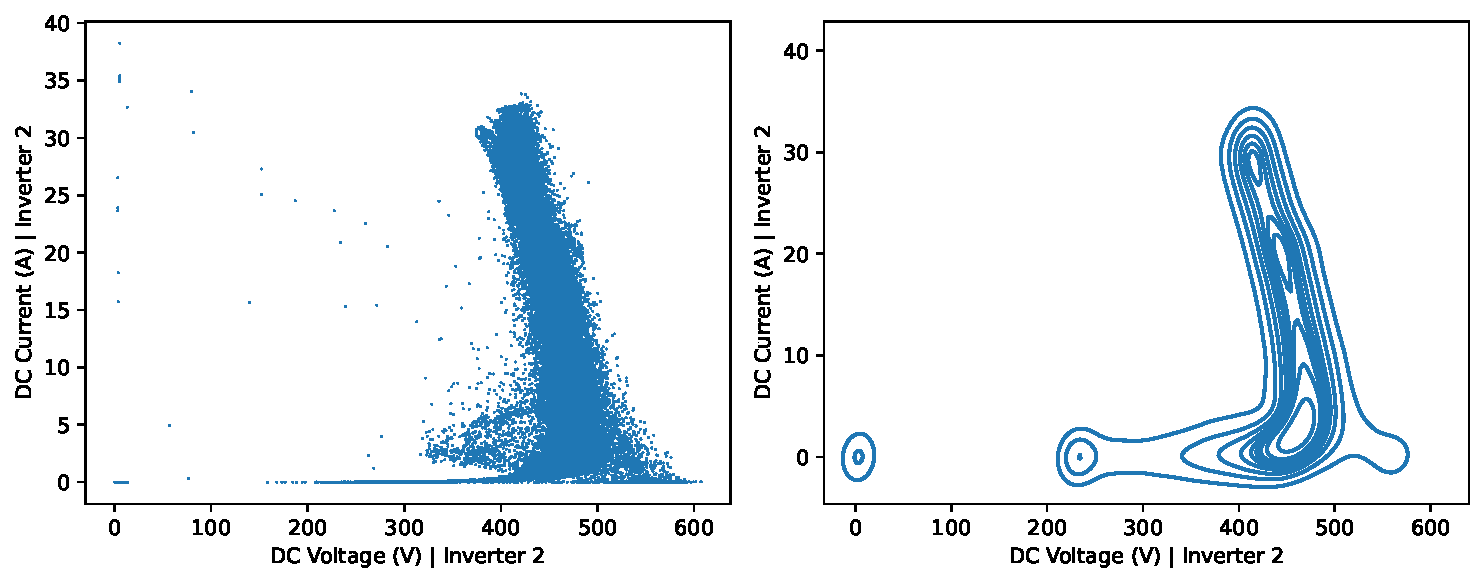
\includegraphics[width=\textwidth]{figures/chapter5/analysis/06_voltage_current_pairplot_kb_2.pdf}
    \caption{\dots}
    \label{fig:eda_volt_curr_pair_kb_2}
\end{figure}

% colocar as figuras disto mas do dataset de teste nos anexos

\dots

\subsubsection{Satellite}

\begin{figure}[h!]
    \centering
    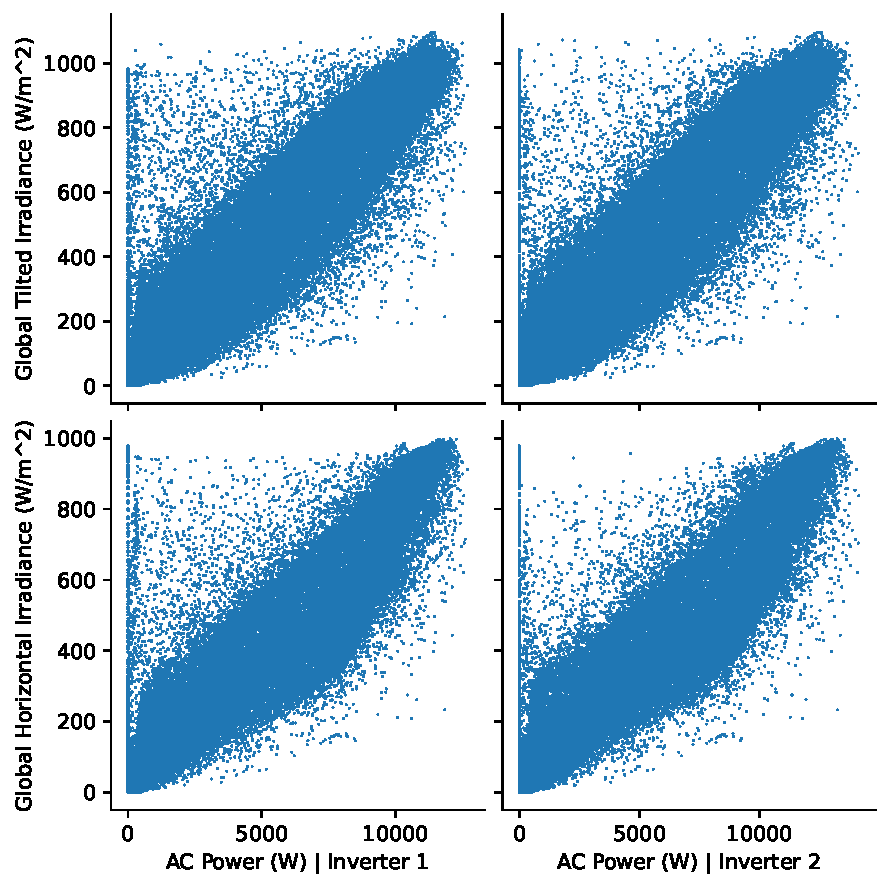
\includegraphics[width=\textwidth]{figures/chapter5/analysis/08_power_irrad_pairplot_scatter_kb.pdf}
    \caption{\dots}
    \label{fig:eda_power_irrad_pair_kb}
\end{figure}
% colocar 09,10,11 nos anexos e mencionar

\begin{figure}[h!]
    \centering
    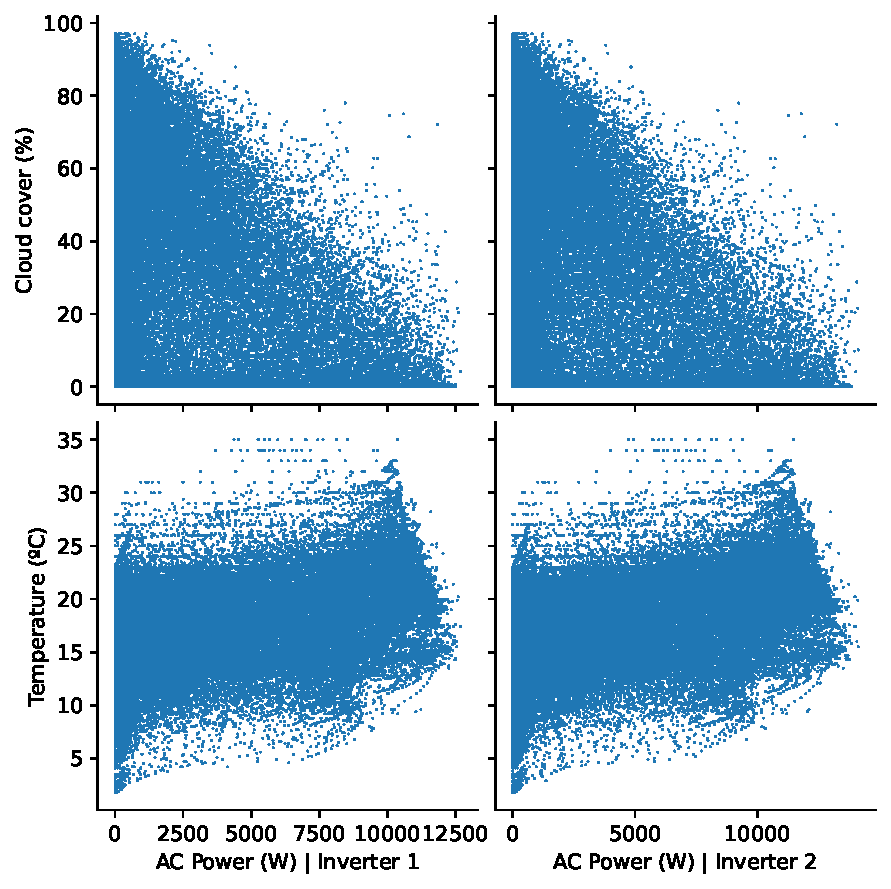
\includegraphics[width=\textwidth]{figures/chapter5/analysis/12_power_meteo_pairplot_kb.pdf}
    \caption{\dots}
    \label{fig:eda_irrelevant_meteo}
\end{figure}

\dots

\subsection{Data Cleaning}

\subsubsection{Power}

% analise e limpeza de dados. Que cenários queremos detetar, o que é que podem ser
\dots

\subsubsection{Satellite}

\dots

\subsubsection{Voltage and Current}

\dots

\subsection{Photovoltaic Plugin}

% formulação do algoritmo para deteçao de falhas em inversores
\dots

\subsection{CellTAN Configuration}

% config das células, como vai correr, como se simula o tempo
\dots

\subsection{Simulation and Results} \label{subsec:results}

\dots

\subsection{Scaling up}

\dots

% \begin{figure}[h!]
%     \centering
%     \includegraphics[width=\linewidth]{figures/chapter4/cell/celltan.pdf}
%     \caption{Ilustrative overview of a CellTAN.}
%     \label{fig:celltan}
% \end{figure}

% Figure \ref{fig:celltan} illustrates a simple CellTAN network overview. Regarding the \textbf{Hub}, one might infer (correctly) that a central component breaks the non-centralized paradigm. Nevertheless, it is present to solve some real-life implementation challenges and limitations, as will be further discussed in this chapter.
